% =====================================================================
%  Vladyslav Lysiuk — CV, англійська версія.
%  Дослівний переклад cv/Lysiuk_CV.pdf: та сама структура, той самий
%  порядок записів, ті самі кольори (#1F4E79 заголовки, #0563C1 посилання)
%  і шрифт Arial.
%
%  Збірка:  xelatex -interaction=nonstopmode Lysiuk_CV_EN.tex
% =====================================================================
\documentclass[11pt,a4paper]{article}

\usepackage{fontspec}
\usepackage[a4paper,left=20mm,right=20mm,top=15mm,bottom=18mm]{geometry}
\usepackage{xcolor}
\usepackage{graphicx}
\usepackage{enumitem}
\usepackage{array}
\usepackage{colortbl}
\usepackage{tabularx}
\usepackage[hidelinks]{hyperref}
\usepackage{xurl}          % довгі посилання переносяться, а не лізуть у поле
\usepackage{microtype}
\usepackage{needspace}     % щоб заголовок не лишався сам унизу сторінки
\sloppy                    % краще трохи ширші пробіли, ніж вихід за поле

\setmainfont{Arial}[
  BoldFont       = Arial Bold,
  ItalicFont     = Arial Italic,
  BoldItalicFont = Arial Bold Italic
]

\definecolor{head}{HTML}{1F4E79}   % заголовки розділів і лінія під ними
\definecolor{link}{HTML}{0563C1}   % посилання
\definecolor{grid}{HTML}{7F7F7F}   % рамка таблиці мов

\hypersetup{colorlinks=true, urlcolor=link, linkcolor=link,
            pdftitle={Vladyslav Lysiuk — CV},
            pdfauthor={Vladyslav Lysiuk},
            pdfsubject={Electronics design engineer (Hardware / PCB Design)}}

\urlstyle{same}            % посилання тим самим шрифтом, а не машинописним
\frenchspacing             % після крапки звичайний пробіл, як у Word
\setlength{\parindent}{0pt}
\setlength{\parskip}{0pt}
\renewcommand{\baselinestretch}{1.06}
\pagestyle{empty}

% ---------- Розділ: синій заголовок і лінія під ним ----------
\newcommand{\heading}[1]{%
  \par\vspace{10pt}%
  \noindent{\color{head}\bfseries\fontsize{13}{15}\selectfont #1}%
  \par\vspace{1pt}%
  \noindent{\color{head}\rule{\linewidth}{0.9pt}}%
  \par\vspace{3pt}%
}

% ---------- Запис: назва ліворуч, дати праворуч (дата не розривається) ----------
\newcommand{\entry}[2]{%
  \par\vspace{5pt}%
  \noindent\begin{tabularx}{\linewidth}{@{}>{\raggedright\arraybackslash\bfseries}X @{\hspace{8pt}}>{\raggedleft\arraybackslash\itshape}p{39mm}@{}}
    #1 & #2
  \end{tabularx}%
  \par\vspace{1pt}%
}

% ---------- Підзаголовок запису (організація, програма) ----------
\newcommand{\org}[1]{{\itshape\raggedright #1\par}\vspace{2pt}}

% ---------- Список пунктів ----------
\newenvironment{points}
  {\begin{itemize}[leftmargin=14pt, itemsep=1.5pt, topsep=2pt, parsep=0pt,
                   label=\textbullet]}
  {\end{itemize}}

\newcommand{\note}[1]{\vspace{2pt}#1\par}

\begin{document}
\fontsize{10}{12.4}\selectfont

% =====================================================================
%  Шапка
% =====================================================================
\begin{minipage}[t]{0.76\linewidth}
  \vspace{0pt}
  \centering
  {\bfseries\fontsize{17}{20}\selectfont LYSIUK VLADYSLAV PAVLOVYCH}\\[3pt]
  {\fontsize{9.5}{11}\selectfont Electronics design engineer (Hardware / PCB Design)}
\end{minipage}%
\hfill
\begin{minipage}[t]{0.22\linewidth}
  \vspace{-6pt}
  \raggedleft
  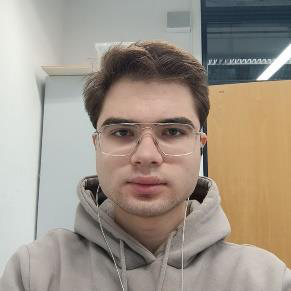
\includegraphics[width=32mm]{../assets/photo.png}
\end{minipage}

\vspace{6pt}
\begin{minipage}[t]{0.74\linewidth}
Location: Chernihiv, Ukraine\\
E-mail: \href{mailto:vladik201611@gmail.com}{vladik201611@gmail.com}\\
Phone: +380685202741\\
Date of birth: 01.04.2005
\end{minipage}

% =====================================================================
\heading{About me}

Junior electronics design engineer. Experience across the full device development cycle:
design of electrical schematic diagrams, creation of component libraries in Altium Designer,
placement and routing of printed circuit boards, assembly and soldering of prototypes,
bring-up, test firmware for STM32 and Arduino Uno microcontrollers. Simulation in Micro-Cap,
Ansys (PyAEDT) and MATLAB. Participant of the international projects Erasmus+ (DIGITRANS),
DAAD Eastern Partnerships and Horizon Europe (NGI~Search). Bachelor's degree with honours.

% =====================================================================
\heading{Education}

\entry{Bachelor (degree with honours) --- 172 Telecommunications and Radio Engineering}{09.2022 -- 06.2026}
\org{Chernihiv Polytechnic National University, Chernihiv, Ukraine}
\begin{points}
  \item Topic of the final qualification work: “Solenoid valve control system with wireless data exchange”.
  \item Within the diploma I performed circuit calculations, printed circuit board routing,
        microcontroller firmware and simulation in MATLAB (the circuit design came from the
        academic supervisor, the work was carried out under his guidance).
  \item Level 6 EQF / NQF.
\end{points}

% =====================================================================
\heading{Project, research and engineering experience}

\entry{Hardware part of the remote power electronics laboratory (LabDiscoveryEngine)}{2023 -- 2024}
\org{Chernihiv Polytechnic National University (within the NGI Search project, Horizon Europe, project No.~101069364)}
\begin{points}
  \item Creation of component libraries and drawing of electrical schematic diagrams in Altium Designer.
  \item Placement and routing of the power electronics printed circuit board under a lecturer's supervision.
  \item Assembly and soldering of the boards; the assembled benches are still in use in the
        university's teaching process.
\end{points}
\note{The results of the work were published in the proceedings of the conference
“Youth Science --- 2024”, page 1039
\url{http://ir.stu.cn.ua/handle/123456789/30262}.}

\entry{Hardware part of the remote microprocessor technology laboratory (Erasmus+ DIGITRANS)}{2024 -- 2025}
\org{EACEA, Erasmus+ Capacity Building, project No.~101127683 --- DIGITRANS}
\begin{points}
  \item Development of a shield (expansion board) for the STM32 NUCLEO-H723 bench: component
        libraries, work with schematics, independent placement and routing of the board.
  \item Testing and soldering of the boards.
  \item Assembly and connection of the benches (Nucleo + Raspberry Pi + Analog Discovery);
        the benches are in use at the university.
  \item Test firmware for the microcontroller: LED control and output of information to a
        7-segment display with multiplexing driven by external signals.
  \item The results were published in the proceedings of the conference NTSS-2024, page 102\\
        \url{http://ir.stu.cn.ua/handle/123456789/32382}
\end{points}
\note{Performer profile: \url{https://hub.stu.cn.ua/project-performer/lysyuk-vladyslav-pavlovych/}}

\entry{Multichannel thermocouple temperature measurement system (DAAD)}{24.10.2024 -- 24.12.2024}
\org{DAAD Eastern Partnerships 2023--2025, “Student Exchange with Online Participation” scholarship}
\begin{points}
  \item Simulation of the analogue path (switching, amplification of the signal of J/K type
        thermocouples) in Micro-Cap.
  \item Calculation of the switching, amplification and filtering circuits, selection of components,
        verification of filtering and switching time under laboratory conditions.
  \item Breadboarding of a 2-channel prototype on a breadboard, control and testing via Arduino.
  \item Reworking of the schematic and the libraries of the existing project of the 24-channel
        measurement board; the following year --- independent routing of the board in Altium Designer.
  \item The results were published in the proceedings of the conference “Youth Science --- 2025”. Page 1012\\
        \url{http://ir.stu.cn.ua/handle/123456789/32545}
\end{points}
\note{Performer profile: \url{https://hub.stu.cn.ua/project-performer/lysyuk-vladyslav-pavlovych/}}

\entry{International internship --- Hochschule Bonn-Rhein-Sieg (H-BRS)}{11.2025 -- 12.2025}
\org{University of Applied Sciences Bonn-Rhein-Sieg, Sankt Augustin, Germany (within DAAD Eastern Partnerships, project No.~57634194)}
\begin{points}
  \item International internship programme (07.11.2025 -- 07.12.2025), certificate of successful completion.\\
        \url{https://drive.google.com/file/d/1uHTCfVhgf4touyQB5vbU6JxceFJbixoN/view?usp=sharing}
  \item Routing of the multichannel temperature measurement board in Altium Designer, routing of
        the board for the qualification work and related engineering tasks.
\end{points}

\entry{Pre-diploma internship --- Hochschule Bonn-Rhein-Sieg (H-BRS)}{05.2026 -- 06.2026}
\org{University of Applied Sciences Bonn-Rhein-Sieg, Sankt Augustin, Germany (DAAD “Eastern Partnership”, project No.~57634194)}
\begin{points}
  \item Pre-diploma internship within short-term academic mobility (02.05 -- 10.06.2026), DAAD grant.
\end{points}

\entry{Research and development in the field of power electronics}{2025 -- 2026}
\org{Department of Electronics, Automation, Robotics and Mechatronics}
\begin{points}
  \item Research on a control algorithm for solenoid valves (three-phase actuation profile) based on
        STM32H743; the results were published in the proceedings of the conference
        “Youth Science --- 2026”. \url{https://ir.stu.cn.ua//handle/123456789/35067} page 1094
  \item Routing of the board of the SIC transistor gate driver module and simulation of the parasitic
        capacitance of the printed circuit board traces in Ansys. The results were published at
        KZYATPS-25, volume 3, page 19
        \url{https://drive.google.com/file/d/1juZTLLvSuyn-di0HTmq1ew8Ju6fRK2ki/view}.
  \item Co-author of a study of ferromagnetic shielding in wireless power transfer systems
        (simulation via PyAEDT/Ansys), publication at the conference “Comprehensive quality
        assurance of technological processes and systems”, 2025.
  \item Performer of the project “Simulation and optimisation of activation capacitors for hybrid
        dynamic wireless power transfer systems” (competition of research works of young scientists).
  \item Bachelor's qualification work: “Solenoid valve control system with wireless data exchange”
        --- independent development of the board, the controller firmware and the MATLAB model
        (see the section “Education”).
\end{points}

% =====================================================================
\heading{Publications}

\begin{points}
  \item V.~P.~Lysiuk and M.~A.~Khomenko, “Multichannel temperature measurement using J and K type
        thermocouples," in XV International Scientific-Practical Conference of students, postgraduates
        and young scientists “YOUTH SCIENCE --- 2025”, Chernihiv, Ukraine: Chernihiv Polytechnic
        National University, 2025, p.~1012.
  \item V.~P.~Lysiuk, M.~A.~Khomenko, "Hardware part of the remote power electronics laboratory based
        on the LabDiscoveryEngine system" --- Youth Science --- 2024, Chernihiv, 2024, p.~1039.
  \item V.~P.~Lysiuk and M.~A.~Khomenko, "Hardware part of the remote laboratory of microprocessor
        technology," in The latest technologies of modern society NTSS-2024, Chernihiv, Ukraine:
        Chernihiv Polytechnic National University, 2024, p.~102.
  \item B.~Pakhaliuk, V.~Lysiuk, and O.~Husev, "Analysis of ferromagnetic shielding patterns in wireless
        power transfer applications using the PyAEDT library in Ansys," in Comprehensive quality
        assurance of technological processes and systems, May 2025.\\
        {\footnotesize\url{https://www.researchgate.net/publication/392126449_Analysis_of_ferromagnetic_shielding_patterns_in_wireless_power_transfer_applications_using_the_PyAEDT_library_in_Ansys}}
  \item B.~Pakhaliuk, V.~Lysiuk, I.~Burmaka, O.~Matiushkin, and R.~Strzelecki, "Simulation analysis of
        wireless power transfer solutions with hybrid inductive and capacitive coupling," in XX
        International Conference MODS 2025: Mathematical and Simulation Modelling of Systems, 2025.
  \item L.~A.~Yarmolenko, V.~P.~Lysiuk, and B.~P.~Pakhaliuk, "Experimental determination of the growth
        rate of a copper electrolytic coating for a 3D printed air capacitor," in The latest technologies
        of modern society (NTSS-2025), Chernihiv, Ukraine, 2025.
  \item V.~Lysiuk, B.~Pakhaliuk, A.~Strohii, L.~Yarmolenko, "Development of an optimized PCB topology
        for a SIC gate driver in a hybrid dynamic wireless power transfer system," Chernihiv Polytechnic
        National University, Chernihiv, 2026, p.~19.
  \item V.~P.~Lysiuk, M.~A.~Khomenko, "Multichannel solenoid valve control device" ---
        Youth Science --- 2026, Chernihiv, 2026.
\end{points}

% =====================================================================
\heading{Grants and international programmes}

\begin{points}
  \item Horizon Europe, NGI Search (HORIZON-CL4-2021-HUMAN-01), project No.~101069364 ---
        participant in the development of the hardware part.
  \item Erasmus+ (EACEA), project No.~101127683 DIGITRANS --- development of the equipment of the
        remote laboratory.
  \item DAAD Eastern Partnerships 24.10.2024 -- 24.12.2024 --- “Student Exchange with Online
        Participation” scholarship (900~EUR).
  \item DAAD “Eastern Partnership”, project No.~57634194 --- academic mobility to Hochschule
        Bonn-Rhein-Sieg (07.11.2025 -- 07.12.2025, grant 861~EUR).
  \item DAAD “Eastern Partnership”, project No.~57634194 --- academic mobility to Hochschule
        Bonn-Rhein-Sieg (02.05 -- 10.06.2026, grant 1342~EUR).
\end{points}

% =====================================================================
\heading{Awards}

\begin{points}
  \item Bachelor's degree with honours (2026).
  \item Letter of appreciation from the Mayor of Chernihiv (May 2024) --- for a significant personal
        contribution to strengthening cooperation at the European level and to the development of
        democratic values, on the occasion of Europe Day
        (\url{https://rtes.stu.cn.ua/2024/05/16/europa-day-event/}).
\end{points}

% =====================================================================
\heading{Technical skills}

\begin{points}
  \item Circuit design and layout: development of electrical schematic diagrams; Altium Designer
        (component libraries, schematics, placement, board routing, including power electronics).
  \item Simulation: Micro-Cap, Ansys / PyAEDT (electromagnetic simulation, parasitic parameters),
        MATLAB/\allowbreak Simulink.
  \item Embedded systems: STM32, Arduino; C for microcontrollers; work with UART, PWM, ADC, I2C, SPI.
  \item Hands-on: assembly and soldering (THT/SMD), breadboarding, with the use of measurement equipment.
\end{points}

% =====================================================================
\Needspace*{8\baselineskip}
\heading{Languages}

\vspace{2pt}
{\fontsize{9}{11}\selectfont
\setlength{\arrayrulewidth}{0.4pt}
\arrayrulecolor{grid}
\begin{tabular}{|l|c|c|c|c|c|}
\hline
 & \multicolumn{2}{c|}{Understanding} & \multicolumn{2}{c|}{Speaking} & Writing \\
\hline
 & Listening & Reading & Spoken interaction & Spoken production & \\
\hline
\textbf{Ukrainian} & C2 & C2 & C2 & C2 & C2 \\
\hline
\textbf{Russian}   & C2 & C2 & C2 & C2 & C2 \\
\hline
\textbf{English}   & B2 & B2 & B1 & B1 & B1 \\
\hline
\end{tabular}
\arrayrulecolor{black}
}

\end{document}
